% !TEX root = 0_main.tex
\chapter{Preliminaries and Background}\label{chap:prelim}
In this chapter, we provide a short background about secure multi-party computation and the generalized problem of \acrfull{sfe}.
Next, we introduce an important special case of two-party \acrshort{sfe} problem and how Yao's \acrfull{gc} protocol can solve it.
Then, we explain basics about combinational and sequential Boolean circuits that are used in the \acrshort{gc} protocol to describe functions.

\section{Secure Multi-party Computation}\label{sec:prelim-smc}
In a secure multi-party computation problem, a number of mutually suspicious parties wish to compute a joint function of their private attributes.
For example, a group of people wants to find their average salary while keeping their salary secret.
The parties have to use some distributed protocols to evaluate and learn the output of the function.
Besides the information that parties can deduce from the output, no other information should leak about the private attributes through the computation.

If there was a third party that all the involving parties trust, they could send their attributes to her, and she computes the function and then returns the result to the parties.
This model is called the ideal model for secure multi-party computation.
Of course, such a trusted party is not available in real scenarios of distributed systems.
Thus at best, the trusted third party can be emulated using a cryptographic protocol (the real model)~\cite{goldreich2013general}.
\fig{fig:multi-party-model} illustrates the idea model with a trusted third party and its emulation in the real model using a secure multi-party computation protocol.

\begin{figure}
    \centering
    \begin{subfigure}[tl]{0.3\textwidth}
        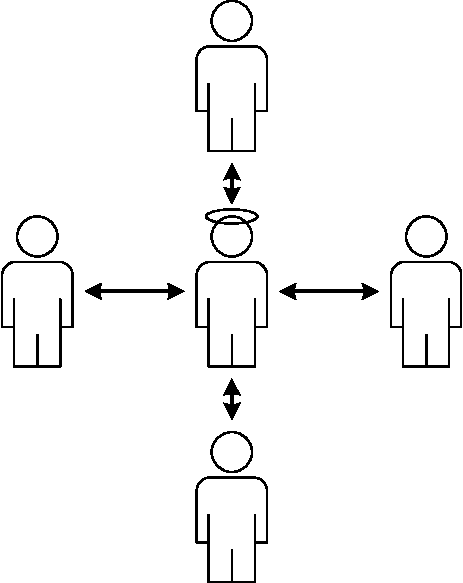
\includegraphics[width=\textwidth]{emulate_ideal-crop.pdf}
        \caption{Ideal Model}\label{fig:ideal-model}
    \end{subfigure}
		~~~~
    \begin{subfigure}[tr]{0.3\textwidth}
        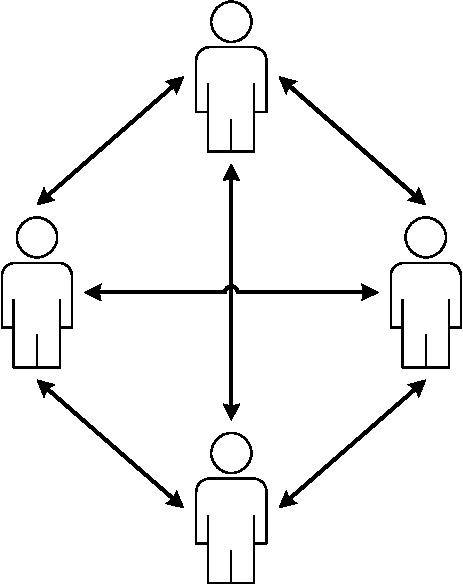
\includegraphics[width=\textwidth]{emulate_real-crop.pdf}
        \caption{Real Model}\label{fig:real-model}
    \end{subfigure}\\
    \caption{Emulation of a trusted third-party in secure multi-party computation (schematic based on~\cite{goldreich2013general}).}\label{fig:multi-party-model}
\end{figure}

\subsection{Secure Function Evaluation}\label{ssec:prelim-sfe}
\acrfull{sfe} is a generic formulation of secure multi-party computation in which parties can evaluate any arbitrary function on their attributes.
Formally in \acrshort{sfe}, there are $p$ parties that have access to secure communication channels between each other.
Each party has an attribute denoted by $i_k$ where $k$ is party identifier.
The parties are interested to collectively compute function $o = f(i_1, i_2, ..., i_p)$ where $f$ is an arbitrary function and $o$ is a tuple $(o_1, o_2, ..., o_p)$ such that $o_k$ belongs to the $k^{\text{th}}$ party.
After the computation of $f$, the parties should gain no information about other parties' attribute, other than the one they can deduce from the output.

We can also  describe the function $f$ as a tuple of functions $f = (f_1, f_2, ...,  f_p)$ where the output of $o_k = f_k(i_1, i_2, .. i_p)$ belongs to $k^{\text{th}}$ party.
A common special case is where $f = f_1 = f_2 = ... = f_p$, meaning all parties receive the same output.
For example in case of the average of salaries, the result of the average function is evaluated and shared with all the participating parties.

\section{Two-Party Secure Function Evaluation}\label{sec:prelim-2sfe}
Two-party \acrshort{sfe} is an important special case of general secure multi-party computation that was introduced and solved by Andrew Yao in his seminal work \cite{yao1986generate}.
In this problem, there are two parties: Alice and Bob; each has an attribute (input) $a$ and $b$ and they want to compute $(o_1, o_2) = (f_1(a, b), f_2(a, b))$ where $o_1$ belong to Alice and $o_2$ belongs to Bob and $f_1$ and $f_2$ are arbitrary polynomial-time computable functions.
\fig{fig:two-party-sfe} illustrates the real model for two-party \acrshort{sfe}.

\begin{figure}
\centering
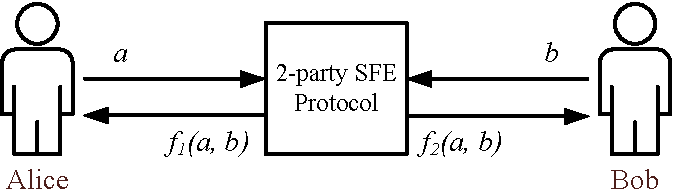
\includegraphics[width=0.70\textwidth]{two_party_SFE-crop.pdf}
\caption{The real model for two-party \acrfull{sfe}.}
\label{fig:two-party-sfe}
\end{figure}

In the following, we explain how the problem of two-party \acrshort{sfe} can be solved using Yao's \acrfull{gc} protocol.
First, we introduce the adversary model supposed for the \acrshort{gc} protocol.
Next, we describe an important cryptographic primitive called Oblivious Transfer used in the \acrshort{gc} protocol.
Then, we explain Yao's \acrshort{gc} protocol and its recent improvements.

\subsection{Adversary Model}\label{ssec:prelim-adv}
We assume that all the parties are semi-honest which means that they follow the protocol exactly as specified without deviation or malicious behavior but they try to learn as much as possible about the other party's input from the information they receive during the protocol.
This model is often called \acrfull{hbc} adversary model in the literature and it is the basis for building a stronger security protocol.
This model can be generalized to more advanced adversary models that are typically addressed by cut-and-chose methods through multiple runs of the basic \acrshort{hbc} model~\cite{lindell2007efficient, lindell2012secure, nielsen2009lego}.

\subsection{Oblivious Transfer}\label{ssec:prelim-ot}
\acrfull{ot}~\cite{naor2005computationally} is a cryptographic protocol based on asymmetric cryptography executed between two parties: Alice (sender) and Bob (receiver).
Through \acrshort{ot}, Bob selects and receives a number of messages from a set provided by Alice without revealing his selection to her.
In a special case of $1$-out-of-$2$ \acrshort{ot} protocol ($\textrm{OT}^2_1$), Alice holds a pair of messages $(m_{0}, m_{1})$; Bob holds a selection bit $b \in \{0, 1\}$ and obtains $m_{b}$ without revealing $b$ to Alice and learns nothing about $m_{1-b}$.

\subsection{Yao's Garbled Circuit Protocol}\label{ssec:prelim-gc}
Yao's Garbled Circuit protocol~\cite{yao1986generate} allows two parties Alice, called the \textit{Garbler} and Bob, called the \textit{Evaluator}, to jointly compute a function $(o_{Alice}, o_{Bob}) = f(a, b)$ on their private attributes (inputs) $a$, provided by Alice and $b$, provided by Bob such that none of them reveal their inputs to each other.
In the end, Alice learns $o_{Alice}$ and Bob learns $o_{Bob}$.
The steps of Yao's protocol are described below.

\begin{enumerate}[label=\roman*.]
\item The function $f$ to be computed is represented as a Boolean circuit, called \textit{\gls{netlist}}, consisting of 2-input 1-output logic gates (a four entry truth table).
\item For each wire $w$ in the \gls{netlist}, Alice assigns two $k$-bit random strings, called \textit{labels}, $X_w^{0}$ and $X_w^{1}$ respectively corresponding to 0 and 1 Boolean values.
      $k$ is the security parameter -- typically $k=128$ is sufficient~\cite{bellare2013efficient}.
\item For each gate, she encrypts the output label in each on of the four rows of the truth table with the corresponding input labels.
      The resulting table of ciphertexts is then randomly rearranged and called the \textit{garbled table}.
\item She then sends the garbled tables along with the labels corresponding to her input values to Bob.
      Bob obtains the labels corresponding to his input values obliviously through 1-out-of-2 \acrshort{ot} protocol.
\item Bob uses these input labels to decrypt the garbled tables gate by gate.
      The label for the output wire of one gate are the label(s) for the input wire(s) of the subsequent gate(s).
\item In the end, Bob learns the labels for the final output wire and Alice has its mapping to 0 and 1.
      Alice sends the mapping for $o_{Bob}$ to Bob and Bob sends the labels for $o_{Alice}$ to her, so they can determine the actual value of outputs.
\end{enumerate}

\subsection{Recent Improvements on the GC Protocol}\label{ssec:prelim-imp}
Throughout the last decade, the cryptographic scheme of the \acrshort{gc} protocol has gone through numerous developments.
We describe the most consequential of these improvements here.

\subsubsection{Free XOR}\label{sssec:prelim-freexor}
The most significant optimization to \acrshort{gc} so far is Free XOR proposed in~\cite{kolesnikov2008improved}.
In this optimization, for any wire $w$, Alice only generates the label $X_w^{0}$ and computes the label corresponding to 1 as $X_w^{0}\oplus (R \parallel 1)$ where $\parallel$ represents bit concatenation and
$R$ is a global random ($k-1$)-bit value known only to Alice.
With this convention, the label for the output of an XOR gate with inputs $a$, $b$ and output $o$ can simply be computed as $X_{o} = X_{a} \oplus X_{b}$.
Thus it does not need computation or transfer of the garbled tables and the XOR gate becomes \textit{free}.

\subsubsection{Row Reduction}\label{sssec:prelim-row}
Row Reduction optimization reduces the size of the tables for the non-XOR gates by $25\%$, i.e., three rows of garbled table are needed to transfered between the parties~\cite{naor1999privacy}.
Here, instead of generating a label for the output wire of a gate randomly, the output label is produced as a function of the labels of the inputs.
Alice generates the output label such that the first entry of the garbled table becomes all $0$ and no longer needs to be sent.

\subsubsection{Garbling with a Fixed-key Block Cipher}\label{sssec:prelim-aes}
This method allows to efficiently garble and evaluate non-XOR gates using fixed-key \acrfull{aes} symmetric encryption~\cite{bellare2013efficient}.
In this garbling scheme which is compatible with the Free XOR and Row Reduction techniques, the output label $X_{o}$ is encrypted with the input label $X_{a}$ and $X_{b}$ using the encryption function $E(X_a,X_b,T,X_o) = \pi(K) \oplus K \oplus X_o$, where $K=2X_a\oplus4X_b\oplus T$, $\pi$ is a fixed-key block cipher (e.g., instantiated with \acrshort{aes}), and $T$ is a unique-per-gate number (e.g., gate identifier) called \emph{tweak}.
A comprehensive proof of security for this method is provided in~\cite{bellare2013efficient}.

\subsubsection{Half Gate}\label{sssec:prelim-half}
Zahur et al., proposed the Half Gate technique that utilizes reduces the cost of non-XOR gates by an additional $25\%$, i.e., two rows of garbled tables are needed to transfered between parties\cite{zahur2015two}.
They also prove that this two rows is the lowest cost possible with symmetric encryption, e.g, \acrshort{aes}.
Fewer than two row may only be possible using costly asymmetric encryption.

\section{Boolean Circuits}\label{sec:prelim-circuit}
In \acrshort{sfe}, the parties are able to evaluate an arbitrary function on their private attributes.
In a number of \acrshort{sfe} protocols including Yao's \acrshort{gc}, \acrfull{gmw}~\cite{goldreich1987play}, and \acrfull{bmr}~\cite{beaver1990round}, the function has to be represented as a Boolean circuit.
In this context, a Boolean circuit can be defined as a directed graph where nodes are 2-input Boolean gates (e.g., AND, OR, NOT, XOR, etc.), edges are wires connecting the gates, and their direction is from the output of a gate to the input of another gate.

\subsection{Combinational Boolean Circuits}\label{ssec:prelim-comb}
The circuits that are used in \acrshort{gc} and other circuit-based \acrshort{sfe} protocols are acrylic Boolean circuits.
In digital circuit theory, such a circuit is called \emph{combinational circuit} and defined as a memory-less circuit in which outputs are functions only of inputs, see \fig{fig:combinational}.

\begin{figure}
    \centering
    \begin{minipage}[t]{0.4\textwidth}
        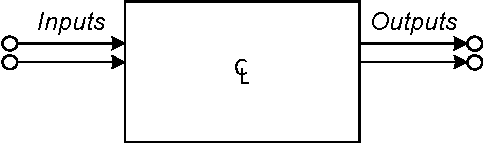
\includegraphics[width=\textwidth]{combinational-crop.pdf}
        \subcaption{Combinational circuit}\label{fig:combinational}
    \end{minipage}
    \begin{minipage}[t]{0.45\textwidth}
        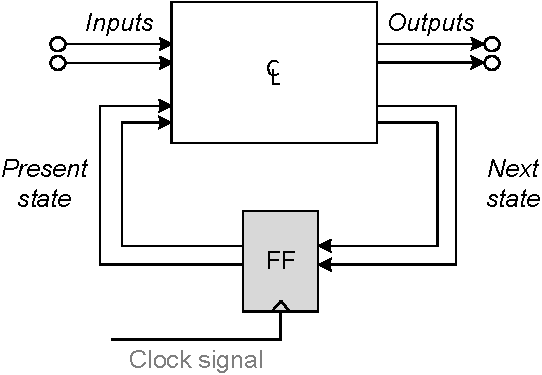
\includegraphics[width=\textwidth]{sequential-crop.pdf}
        \subcaption{Sequential circuit}\label{fig:sequential}
    \end{minipage}\\
    \caption{(a) Combinational circuit where outputs are functions of only inputs. (\acrfull{cl} represents \acrlong{cl}.)
    (b) Sequential circuit where outputs are functions of inputs and present states.
    }\label{fig:combinational-sequential}
\end{figure}

\subsection{Sequential Boolean Circuits}\label{ssec:prelim-seq}
Another class of circuits in digital circuit theory are \emph{sequential circuits} in which unlike in combinational, the circuit outputs are functions of both inputs and circuit \emph{states}.
The circuit states are kept in memory elements such as \acrfull{ff}.
The states can change at the end of each \emph{clock cycle}\footnote{The clock signal oscillates between a low and a high state and its (rising) edge is typically utilized to coordinate the memory updates.}.
In this thesis, we use only \acrfull{d-ff}, a type of \acrshort{ff} that has four inputs: D (data), I (initial), clk (clock), and rst (reset) and one output: Q (latched data).

\begin{figure}
    \centering
	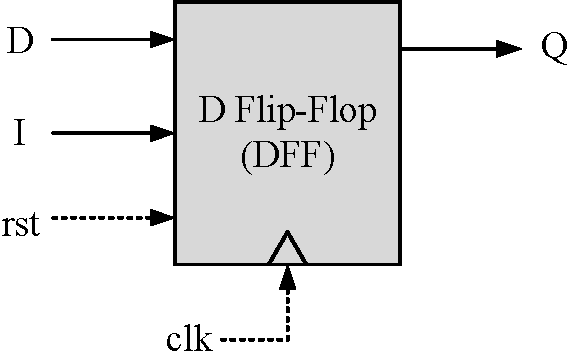
\includegraphics[width=0.4\textwidth]{ff-crop.pdf}
	\caption{Schematic of a \acrshort{d-ff} with initial value.}
	\label{fig:ff}
\end{figure}

As seen in \fig{fig:sequential}, a sequential circuit can be represented as an ensemble of a combinational circuit and feedback loops with memory elements.
At each cycle, circuit inputs as well as the present states are fed to the combinational part.
Then, it generates the outputs and next states which will be stored in the memory elements for the next cycle.
The initial value of the memory elements are either a known constant value ($0$ or $1$) or determined by an initial input value (I).
In a digital hardware, \acrshort{ff} initialization is usually done by \emph{reset} or \emph{set} signals.
In \gls{tinygarble}, signal I of an \acrshort{ff} can be connected to a constant value or input wire (in this cased called \emph{init} wire).
